\subsection{滤波器}

\begin{definition}
    \bd{滤波器}是以特定方式改变信号的频率特性,从而变换信号的处理系统。
    滤波器一般有如下类别,如图 \ref{fig:filter_types} 所示:
    \begin{enumerate}[label=(\arabic*)]
        \item 高通滤波器(HP)
        \item 低通滤波器(LP)
        \item 带通滤波器(BP)
        \item 带阻滤波器(BS)
        \item 全通滤波器(AP)
    \end{enumerate}
    \begin{figure}[H]
        \centering
        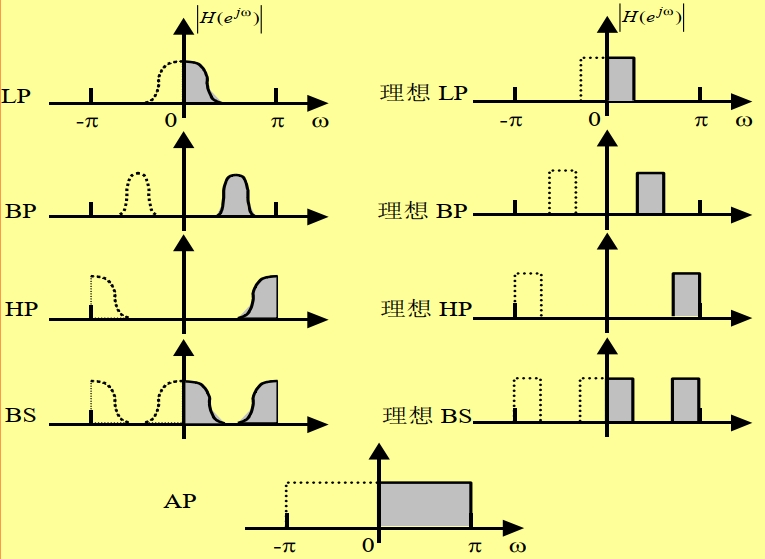
\includegraphics[width=0.8\textwidth]{chap4/img/filter_types.png}
        \caption{滤波器类型}
        \label{fig:filter_types}
    \end{figure}

    滤波器也可以被分为\bd{模拟滤波器}和\bd{数字滤波器}。
    \begin{itemize}
        \item \bd{模拟滤波器}是由电阻、电容、电感等部件构成的电路。
            滤波器特性对所用部件的物理标称值非常敏感,而且,
            有些部件的物理特性会随温度变化而改变。
        \item \bd{数字滤波器}是用软件实现的,很少依赖硬件。滤波软件
            只是一系列程序指令。虽然它是在硬件平台上运行,但
            是硬件平台本身并不决定滤波器的性能。数字滤波器的
            性能是由\bd{一组系数}确定的。
    \end{itemize}
    数字滤波器的实现方式一般有以下几种:
    \begin{enumerate}
        \item 用流图计算滤波器的输出。
        \item 用差分方程计算滤波器的输出。
        \item 用卷积过程计算滤波器的输出。
        \item 用 DTFT 直接改变信号频谱。
    \end{enumerate}
\end{definition}

\begin{definition}
    模拟
\end{definition}

\begin{exercise}
    已知某系统的差分方程如下式:
    \begin{align*}
        y(n) = x(n) + x(n - 3) + 0.7y(n - 1) + 0.6y(n - 2).
    \end{align*}
    \begin{enumerate}[label=(\arabic*)]
        \item 判断系统的脉冲响应类型。
        \item 画出该系统的信号流图。
    \end{enumerate}
\end{exercise}

\begin{solution}
    \begin{enumerate}[label=(\arabic*)]
        \item 该系统的脉冲响应类型为无限脉冲响应。
        \item 该系统的直接 I 型信号流图如图 \ref{fig:signal_flow_diagram} 所示。
            \begin{figure}[H]
                \centering
                \tikzstyle{block} = [draw, rectangle, minimum height=1cm, minimum width=1cm]
                \tikzstyle{circ} = [draw, fill, circle, inner sep=1.5pt]
                \tikzstyle{sum} = [draw, circle]
                \tikzstyle{line} = [draw, -latex]
                \tikzstyle{no-arrow-line} = [draw, -]
                \tikzstyle{gain} = [draw, isosceles triangle, isosceles triangle apex angle=60, shape border rotate=180]
                \begin{tikzpicture}

                    \node [name=input] (input) {$x(n)$};
                    \node [circ, right of=input, xshift=1cm] (circ1) {};
                    \node [sum, right of=circ1, xshift=4cm] (sum) {$+$};
                    \node [block, below of=circ1, yshift=-2cm] (d1) {$Z^{-1}$};
                    \node [block, below of=d1, yshift=-2cm] (d2) {$Z^{-1}$};
                    \node [block, below of=d2, yshift=-2cm] (d3) {$Z^{-1}$};
                    \node [circ, right of=sum, xshift=4cm] (circ2) {};
                    \node [name=output, right of=circ2, xshift=1cm] (output) {$y(n)$};
                    \node [block, below of=circ2, yshift=-2cm] (d4) {$Z^{-1}$};
                    \node [block, below of=d4, yshift=-2cm] (d5) {$Z^{-1}$};
                    \node [circ, below of=d4, yshift=-0.5cm] (circ3) {};
                    \node [gain, below of=d4, xshift=-2cm, yshift=-0.5cm] (g1) {$0.7$};
                    \node [gain, below of=d5, xshift=-2cm, yshift=-0.5cm] (g2) {$0.6$};

                    \path [no-arrow-line] (input) -- (circ1);
                    \path [line] (circ1) -- (sum);

                    \path [line] (circ1) -- (d1);
                    \path [line] (d1) -- (d2);
                    \path [line] (d2) -- (d3);
                    \path [line] (d3.east) -- (sum);

                    \path [no-arrow-line] (sum) -- (circ2);
                    \path [line] (circ2) -- (output);

                    \path [line] (circ2) -- (d4);
                    \path [no-arrow-line] (d4) -- (circ3);
                    \path [line] (circ3) -- (g1);
                    \path [line] (circ3) -- (d5);
                    \path [line] (d5) |- (g2);

                    \path [line] (g1.west) -- (sum);
                    \path [line] (g2.west) -- (sum);
                \end{tikzpicture}
                \caption{信号流图}
                \label{fig:signal_flow_diagram}
            \end{figure}
    \end{enumerate}
\end{solution}
